\documentclass[border=6pt]{standalone}
\usepackage{amsmath}
\usepackage{tikz}
\usetikzlibrary{positioning, arrows.meta, fit, backgrounds, calc}
\tikzset{stage/.style={draw, rounded corners, align=center, font=\small, minimum height=1.0cm, minimum width=2.6cm, thick},
layer/.style={draw, dashed, rounded corners, inner sep=10pt},
node_t/.style={draw, circle, align=center, font=\scriptsize, minimum size=1.0cm, thick},
flow/.style={-{Stealth[length=2.5mm]}, thick},
edge_t/.style={-{Stealth[length=2mm]}, font=\scriptsize}}
\begin{document}
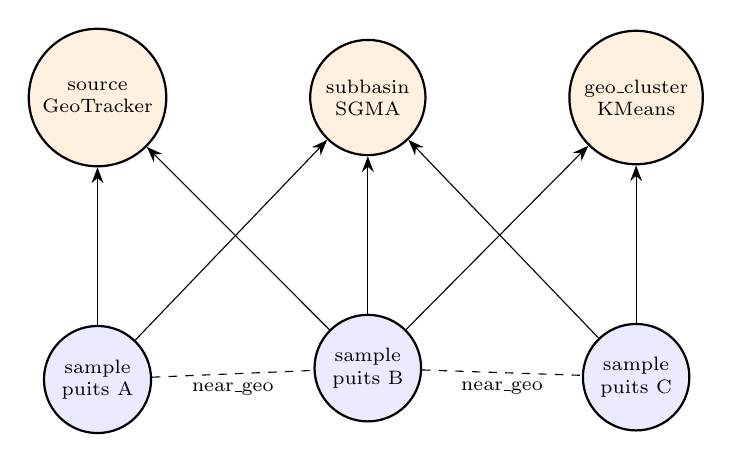
\begin{tikzpicture}[node distance=1.5cm and 1.8cm]
  % hubs
  \node[node_t, fill=orange!12] (src) {source\\ GeoTracker};
  \node[node_t, fill=orange!12, right=of src] (sub) {subbasin\\ SGMA};
  \node[node_t, fill=orange!12, right=of sub] (clu) {geo\_cluster\\ KMeans};
  % samples
  \node[node_t, fill=blue!8, below=2cm of src] (s1) {sample\\ puits A};
  \node[node_t, fill=blue!8, below=2cm of sub] (s2) {sample\\ puits B};
  \node[node_t, fill=blue!8, below=2cm of clu] (s3) {sample\\ puits C};
  % belongs
  \draw[edge_t] (s1) -- (src); \draw[edge_t] (s2) -- (src);
  \draw[edge_t] (s1) -- (sub); \draw[edge_t] (s2) -- (sub); \draw[edge_t] (s3) -- (sub);
  \draw[edge_t] (s2) -- (clu); \draw[edge_t] (s3) -- (clu);
  % near_geo (sample<->sample)
  \draw[dashed] (s1) -- node[below,font=\scriptsize]{near\_geo} (s2);
  \draw[dashed] (s2) -- node[below,font=\scriptsize]{near\_geo} (s3);
\end{tikzpicture}

\end{document}
